\documentclass[slovak, master]{diploma}

% Packages (balíky makier)
\usepackage[autostyle=true, czech=quotes]{csquotes} % korektná sadzba úvozoviek, podpora pre balík biblatex
\usepackage[backend=biber, style=iso-numeric, alldates=iso]{biblatex} % bibliografia
\usepackage{dcolumn} % stĺpce tabuľky s číselnými hodnotami
\usepackage{subfig} % makrá pre "podobrázky" a "podtabuľky"
\usepackage[csharp]{diplomalst} % sádzanie
\usepackage{svg}
%\usepackage[python]{diplomalst}
%\usepackage{tcolorbox} % oramovanie

% ------------------------------------------------------

% Definované vlastné metódy, triedy a príslušné farby
% viz bakalarka

% ------------------------------------------------------

% Nový druh tabuľkového stĺpca, v ktorom sú čísla zarovnané podľa desetinnej čiarky
\newcolumntype{d}[1]{D{,}{,}{#1}}

% Odstranenie warningov s underfull vbox
\raggedbottom

% Nastavenie tex color boxu
%\newtcbox{\mybox}[2][black]{outer arc=0pt,  boxsep=0pt, left=0pt, right=0pt, top=0pt, bottom=0pt, boxrule=2pt}

% ------------------------------------------------------

%Zásady pro vypracování
% S umělou inteligencí, která je zodpovědná za rozhodování, se setkáme ve většině počítačových her, ať už jde o hry deskové, plošinové nebo např. tahové. Cílem této diplomové práce je naimplementovat herní prostředí, v němž budou pro rozhodování použity klasické algoritmy jako např. ID3, C4.5, CART (regresní stromy), CHAID (Chi-square, automatic interaction detection), MARS ( (multivariate adaptive regression splines), náhodný les (random forest) a algoritmy jako Deep Q-learning, Double Deep Q-learning, popř. hluboké neuronové sítě a tyto metody porovnat na základě experimentů a následné statistické analýzy. Metody budou porovnány na základě výkonu a úspěšnosti z hlediska řešení daných problémů.

% Zásady pro vypracování:
% 1. Seznamte se s algoritmy jmenovanými výše a způsobem jejich použití v počítačových hrách.
% 2. Navrhněte vlastní netriviální počítačovou hru, kde budou vybrané algoritmy použity pro rozhodování tzv. NPC (non-playing character). Při výběru algoritmů je potřeba, aby byly zastoupeny obě kategorie výše zmíněných algoritmů - tzn. klasické i algoritmy strojového učení. Celkem by mělo být použito aspoň 5 algoritmů, kde aspoň 2 budou patřit do kategorie strojového učení. Ve hře bude implementována postava hráče, který bude proti NPC bojovat.
% 3. Naimplementujte zvolené algoritmy a proveďte jejich srovnání na základě opakovaných experimentů. Během implementace klaďte důraz na efektivitu. Žádný z algoritmů nesmí být proti jinému zvýhodněn. Proveďte statistickou analýzu a s použitím vhodných statistických testů vyhodnoťte kvalitu poskytovaného řešení těchto algoritmů a jejich výkon.
% 4. Výsledky zpracujte v podobě tabulek a grafů a na jejich základě proveďte vyhodnocení testů. Shrňte výhody a nevýhody jednotlivých algoritmů. V závěru uveďte, který algoritmus dosáhl nejlepšího výkonu a který byl při řešení daných úkolů nejúspěšnější.

% ------------------------------------------------------

% Titulná strana
\ThesisAuthor{Bc. Miroslav Kačeriak}
\ThesisSupervisor{prof. Ing. Jan Platoš, Ph.D.}
\CzechThesisTitle{Rozhodování v počítačových hrách - srovnání metod umělé inteligence}
\EnglishThesisTitle{Decision Making in Computer Games - a Comparison of Artificial Intelligence Methods}
\ThesisAssignmentFileName{ThesisSpecification_KAC0067_vsboee22026009.pdf}
\SubmissionYear{2023}

% ------------------------------------------------------

% Abstrakty
\CzechAbstract{TODO}
% po cesky?

\CzechKeywords{spätnoväzobné učenie, rozhodovacie stromy, ID3, D4.5, CART, Unity engine, C\#, Python}

\EnglishAbstract{TODO}

\EnglishKeywords{reinforcement learning, decision trees, ID3, D4.5, CART, Unity engine, C\#, Python}

% ------------------------------------------------------

% Poďakovanie
\Acknowledgement{Rád by som na tomto mieste poďakoval prof. Ing. Jánovi Platošovi, Ph.D. za pomoc a ochotu prejavenú popri vedení tejto diplomovej práce a mojej priateľke Zdenke za trpezlivosť a prínosné rady, bez ktorých by výsledná práca bola o niečo chudšia.}

% ------------------------------------------------------

% Skratky
\AddAcronym{AI}{Artificial intelligence}
\AddAcronym{API}{Application Programming Interface}
\AddAcronym{CART}{Classification and Regression Tree}
\AddAcronym{GUI}{Graphic User Interface}
\AddAcronym{FPS}{Frames Per Second}
\AddAcronym{NPC}{Non-Playable Character}
\AddAcronym{FOV}{Field of view}

% ------------------------------------------------------

% Literatúra
\addbibresource{literature.bib}

% ------------------------------------------------------

% Samotný dokument
\begin{document}
\MakeTitlePages

% Zoznam obrázkov
\listoffigures
\clearpage

% Zoznam tabuliek
\listoftables
\clearpage

% Zoznam zdrojakov
\lstlistoflistings
\clearpage

% Chapter 0
\chapter{Úvod}
\label{sec:Introduction}
%TODO

% ------------------------------------------------------

% Teória
% Chapter 1
\chapter{Umelá inteligencia v hrách}
\label{sec:AI in games}

\chapter{Strojové učenie}
\label{sec:MachineLearningOverview}
%TODO

\section{Rozhodovacie stromy}
\label{sec:DecisionTreesOverview}
%TODO
\subsection{Algoritmus ID3}
\label{sec:ID3}
%TODO
\subsection{Algoritmus D4.5}
\label{sec:D45}
%TODO
\subsection{Algoritmus CART}
\label{sec:CART}
%TODO

\section{Spätnoväzobné učenie}
\label{sec:ReinforcemenLearningOverview}
%TODO

% ------------------------------------------------------

% Vypracovanie
% Chapter 3
\chapter{Použité technológie}
\label{sec:Tech}
%TODO
\section{Unity Engine}
\label{sec:Unity}
%TODO
\section{Programovacie jazyky}
\label{sec:langs}
%TODO + c# + python?
\section{Nástroj ML-Agents}
\label{sec:ML-Agents}
%TODO
\subsection{Inštalácia prvotné nastavenie}
\label{sec:MLAgentsInstall}
%TODO
%...?

% Chapter 4
\chapter{Hra a herné prostredie}
\label{sec:GameOverview}
Táto kapitola je venovaná vytvorenej hre ako takej, všetkým jej aspektom a princípom fungovania. Prvá sekcia si kladie za cieľ popísať žánrové a príbehové zasadenie hry. V ďalších sekciách je potom podrobne prebratá architektúra a fungovanie jednotlivých herných mechaník.

\section{Žáner a príbehové zasadenie}
\label{sec:GenreAndSetting}
Hra samotná má svojou hrateľnosťou najbližšie k žánru stealth. Tento žáner sa vyznačuje tým, že hráč sa snaží vyhnúť odhaleniu a následnému priamemu stretu s nepriateľom. K dosiahnutiu cieľa je teda využívaný pomalý a tichý postup, kde každý krok by mal byť dobre premyslený a načasovaný. 

Príbeh hry je zasadený do pirátskeho prostredia. Hráč sa ocitá v roli radového člena pirátskej posádky, ktorá bola napadnutá flotilou anglického námorníctva. S vypätím všetkých síl sa mu na poškodenom záchrannom člne podarilo dostať na najbližší obývaný ostrov, kde však zisťuje, že nie je všetko v poriadku. Namiesto obyvateľov ostrova nachádza len agresívnych kostlivcov. 

Hráčovou ovláda postavu z pohľadu tretej osoby a jeho úlohou je nájsť na ostrove funkčný čln, pozbierať zásoby nutné na ďalšiu plavbu a pokiaľ možno pri tom nevzbudiť pozornosť.

\begin{figure}[!htbp]
	\centering
	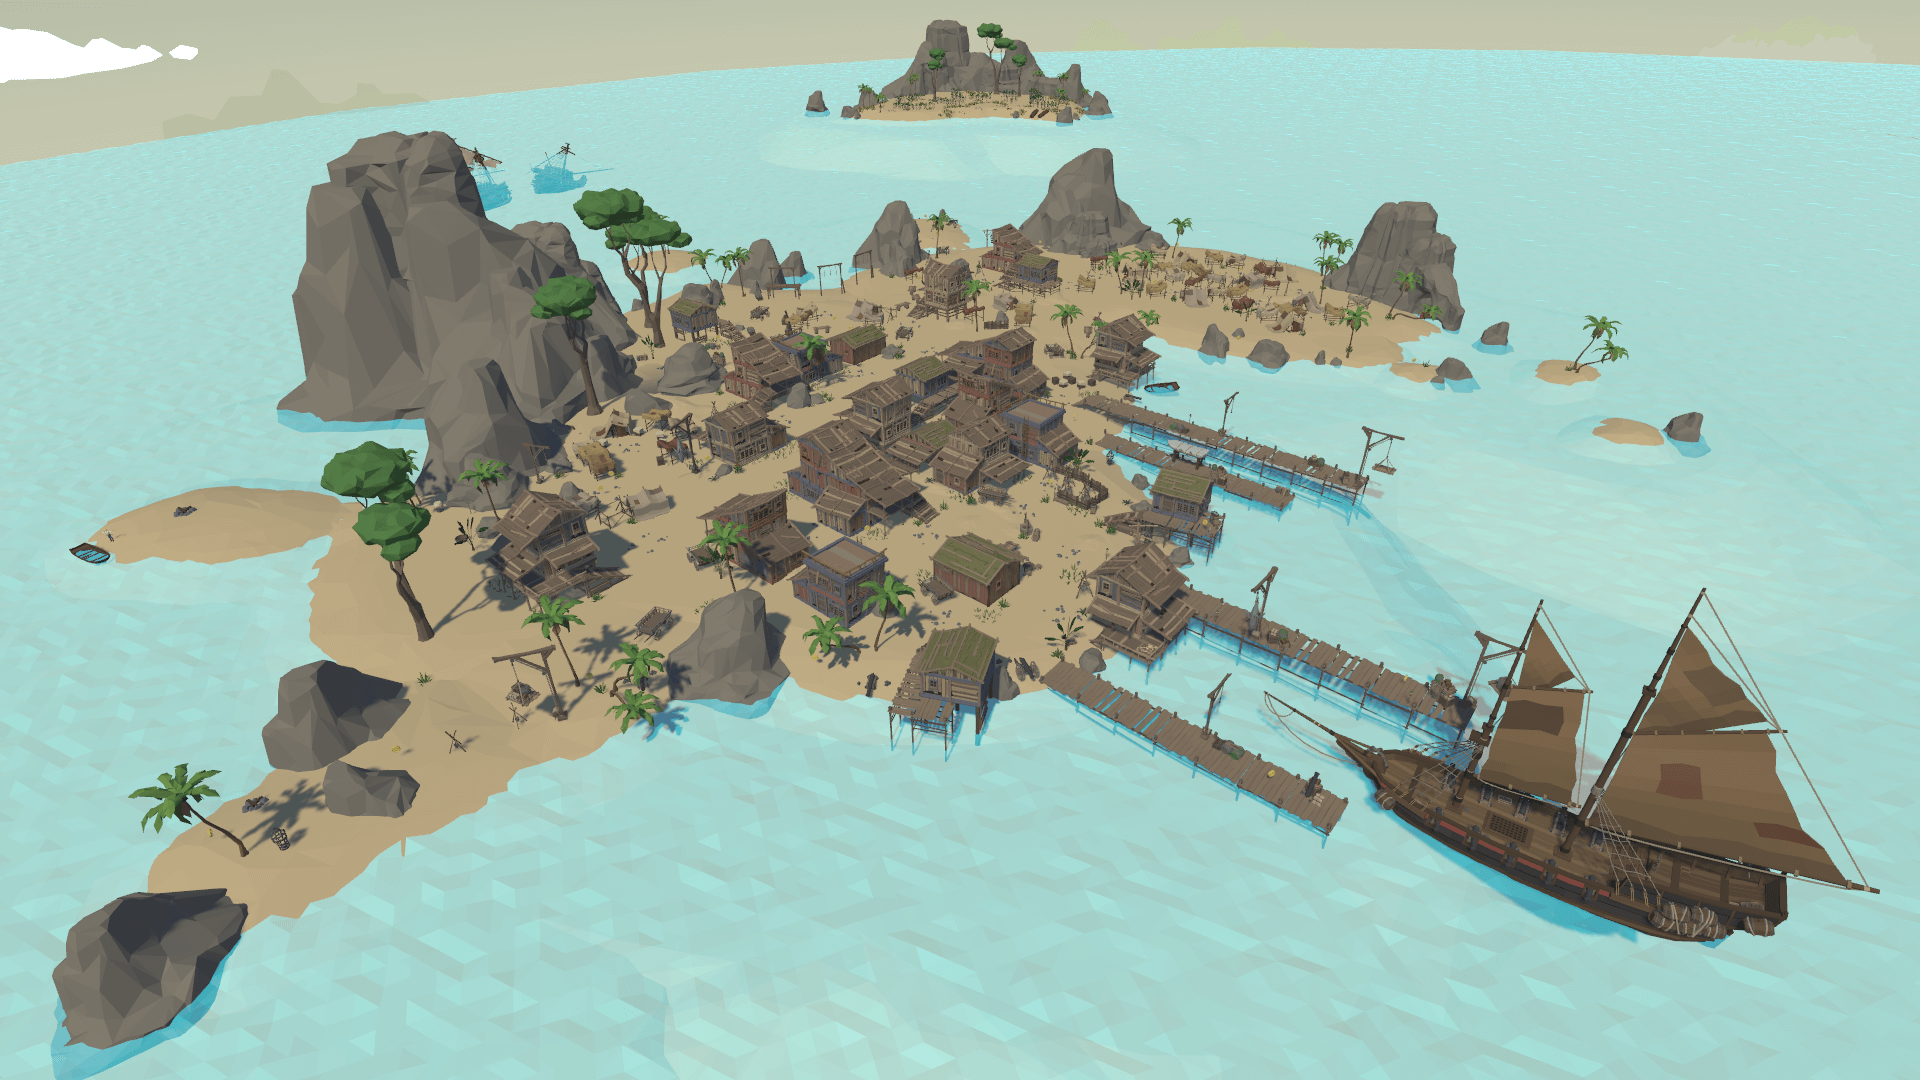
\includegraphics[width=.9\textwidth]{Figures/game_compressed.png}
	\caption{Vyrenderovaná snímka z hry}
	\label{pic:GameScreenshot}
\end{figure}

\section{Architektúra hry}
\label{sec:GameStructure}
%TODO
%spomenut synty tu
%manazeri overview
Hra je rozdelená do dvoch samostatných scén. Konkrétne ide o hlavnú scénu, kde sa odohráva samotná herná slučka a scénu s hlavnou ponukou. V editore Unity je možné medzi jednotlivými scénami ľubovoľne prepínať, prípadne mať aktívnych niekoľko scén naraz. V samostatnom zostavení aplikácie je však nutné vybrať, ktoré konkrétne scény budú prítomné. Každá scéna potom dostane poradové číslo, tzv. build index a scéna s číslom nula, v tomto prípade hlavná ponuka, bude spustená ako prvá. Scéna s hlavnou ponukou je bližšie popísaná v sekcií \ref{sec:MainMenuAndUI}.

Scénu je potom možné chápať ako koreňový adresár pre hierarchiu objektov v hre. Jednotlivé herné objekty je možné vložiť do scény priamo alebo ako potomka iného herného objektu. Manipulácia s pozíciou, rotáciou či mierkou objektu sa teda aplikuje aj na všetkých jeho potomkov. Naopak to však neplatí. Z tohto dôvodu sa rozlišujú dve súradnicové sústavy, a síce globálna (celková) a lokálna (relatívna voči predkovi). Využitie globálnej súradnicovej sústavy však vyžaduje vziať do úvahy parametre všetkých predkov daného objektu v scéne, čo nie je ideálne z hľadiska výkonu. Preto bol v projekte preferovaný lokálny súradnicový systém napríklad u herných NPC agentov či predmetov, ktoré je v hre možné zbierať. Predkovia týchto objektov sú potom umiestnení v počiatku súradnicovej sústavy, čo zaisťuje konzistenciu so zvyškom objektov v scéne.

V každej scéne sa nachádza objekt MainManager, ktorý slúži ako prístupový bod k ostatným manažérom, ktorí spravujú centrálne prvky hry. Tento typ architektúry sa kvôli svojej jednoduchosti často uplatňuje medzi malými až strednými projektami. V tomto projekte sú použité objekty ConfigManager, GameManager, InputManager a SoundManager, nie všetky sú však vyžadované v každej scéne. 

Krátky popis jednotlivých manažérov:
\begin{itemize}
  \item \textbf{ConfigManager} -- je prístupovým bodom k nastaveniam hry, zaisťuje serializáciu a deserializáciu dát, rovnako ako ich perzistentnosť po každej zmene.
  \item \textbf{GameManager} -- reštartuje scénu pri smrti alebo výhre hráča, kontroluje prerekvizity výhry, aktualizuje grafické užívateľské rozhranie pri získaní predmetu a zobrazuje kontextovú ponuku na ukončenie hry či návrat do hlavnej ponuky po stlačení príslušnej klávesy.
  \item \textbf{InputManager} -- centralizuje získavanie užívateľského vstupu z klávesnice, myši, či iných herných periférií, čo umožňuje na jednom centrálnom mieste zamieňať rôzne implementácie, prípadne z testovacích dôvodov hráčsky vstup úplne ignorovať. 
  \item \textbf{SoundManager} -- Vyvoláva jednoduchú simuláciu zvuku, na ktorú môžu zareagovať NPC agenti v dosahu.
\end{itemize}

\section{Herná slučka}
\label{sec:GameLoop}
Tradičná herná slučka definovaná napríklad podľa \cite{GameAlgorithms} sa skladá z troch fáz:

\begin{enumerate}
  \item Spracovanie vstupov
  \item Aktualizácia herného sveta
  \item Generovanie výstupov
\end{enumerate}

Hra teda prijme užívateľský vstup, na základe neho aktualizuje herný svet (dynamické objekty, ktoré sa v ňom vyskytujú) a výsledný stav je potom vyrenderovaný hráčovi v ďalšom snímku. Tento postup sa opakuje niekoľkokrát za sekundu, čo vyvoláva ilúziu dynamického sveta. Dnes sa považuje za štandard vykonanie hernej slučky 30 až 60 krát za sekundu. Dnešný hardvér však už podporuje vykresľovanie aj o rýchlosti 500FPS. Lepšou metrikou pre vývojárov je však tzv. frame time, teda trvanie jednej hernej slučky v ms. Vzťah týchto veličín je znázornený na obrázku \ref{pic:FrameTimeFPS}.

\begin{figure}[!htbp]
	\centering
	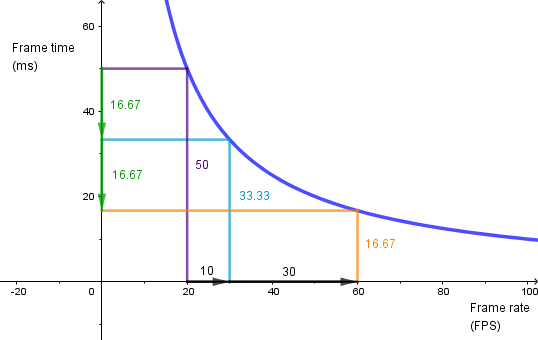
\includegraphics[width=.8\textwidth]{Figures/frameTimeVsFPS.png}
	\caption{Metriky Frame Time a FPS \cite{FrameTimeFPS}}
	\label{pic:FrameTimeFPS}
\end{figure}

V kontexte konkrétnej hry sa však pojem herná slučka alebo základná herná slučka (core game loop) využíva skôr na popis základných herných mechaník. V tomto prípade by teda šlo o prechod z bodu A do bodu B a zozbieranie určitého počtu predmetov na vymedzenej hernej ploche.

Pokiaľ hráčovi klesne život na nulu, hra pre neho končí a vracia sa na počiatočnú lokáciu. Nepriatelia a zberateľné predmety sa vrátia na svoje počiatočné pozície. Ak hráč dôjde do cieľa a splní prerekvizitu výhry, teda má v inventári určitý počet predmetov daného typu, hru vyhráva. 

Základnú hernú slučku obstaráva objekt GameManager spomenutý v sekcií \ref{sec:GameStructure}. Po hernej ploche je ručne rozmiestnených päť fliaš, z ktorých musí hráč nájsť a zobrať aspoň tri a tridsaťpäť mincí, pričom je pre dosiahnutie výhry nutné mať aspoň dvadsaťpäť. 

Implementačne oba typy objektov dedia z triedy Pickup, ktorej telo je možné vidieť vo výpise \ref{src:Pickup}. Tá potom dedí priamo z triedy UnityEngine.MonoBehaviour, čo je bázová trieda, z ktorej dedia musia dediť všetky triedy, ktoré nejakým spôsobom využívajú Unity API \cite{MonoBehaviour}. Typicky ide o metódy ako napríklad Awake(), Start(), Update(), či FixedUpdate(), ktoré sú definované v životnom cykle Unity objektu, ale aj metódy sprístupňujúce prácu s korutinami apod.
\vspace{8pt}
\begin{lstlisting}[label=src:Pickup,caption={Trieda Pickup slúžiaca ako predok všetkých zberateľných predmetov v hre}]
public class Pickup : MonoBehaviour
{
    public event Action<Pickup> OnPickedUp;
    private WaitForEndOfFrame waitForFrameToEnd = new WaitForEndOfFrame();
    private MeshRenderer mesh;

    private void Start() 
    {
        MainManager.Instance.GameManager.RegisterPickup(this);
        mesh = GetComponentInChildren<MeshRenderer>();
    }
    private void OnTriggerEnter(Collider other) 
    {
        if (!other.gameObject.CompareTag(Constants.PlayerTag)) return;

        OnPickedUp?.Invoke(this);
        StartCoroutine(LerpPosition(transform.position, Camera.Instance.PickupTarget.position, 0.2f, () => { gameObject.SetActive(false); }));
    }
    private void OnDestroy() 
    {
        MainManager.Instance.GameManager.UnregisterPickup(this);
    }
    IEnumerator LerpPosition(Vector3 start, Vector3 end, float timeToMove, Action callback) 
    {
        float time = 0;

        while (time < 1)
        {
            mesh.transform.position = Vector3.Lerp(start, end, time);
            time += Time.deltaTime / timeToMove;

            yield return waitForFrameToEnd;
        }

        mesh.transform.position = end;
        callback();
    }
}
\end{lstlisting}

V metóde Start(), teda na začiatku svojho životného cyklu, ktorý sa odohrá po spustení scény sa každý zberateľný objekt zaregistruje v objekte GameManager, čo spôsobí napojenie na event OnPickedUp, a umožní GameManagerovi v správnej chvíli zareagovať na získanie predmetu hráčom a aktualizovať GUI či inventár bez nutnosti periodického dopytovania. Nakoľko je v odberateľovi eventu odosielaná aj daná inštancia objektu, je jednoduché zistiť typ predmetu, ktorý hráč zobral.

Metóda OnTriggerEnter() je potom zavolaná v momente, keď hráčov kontroler začne kolidovať s komponentou box collider daného objektu. K tomu je nutné nastaviť tento box collider ako trigger a zároveň mať na objekte prítomnú komponentu rigidbody, ktorá obstaráva simuláciu fyziky. V tomto momente sa zároveň pomocou korutiny LerpPosition() začne objekt rýchlo pohybovať do pravého horného rohu obrazovky, kde sa nachádza UI element zobrazujúci hráčovi počet zozbieraných predmetov, a následne sa deaktivuje. Tento efekt bol často využívaný v starších 2D platformových hrách. Zberateľný predmet je možné vidieť na obrázku \ref{pic:Pickup}.

\begin{figure}[!htbp]
	\centering
	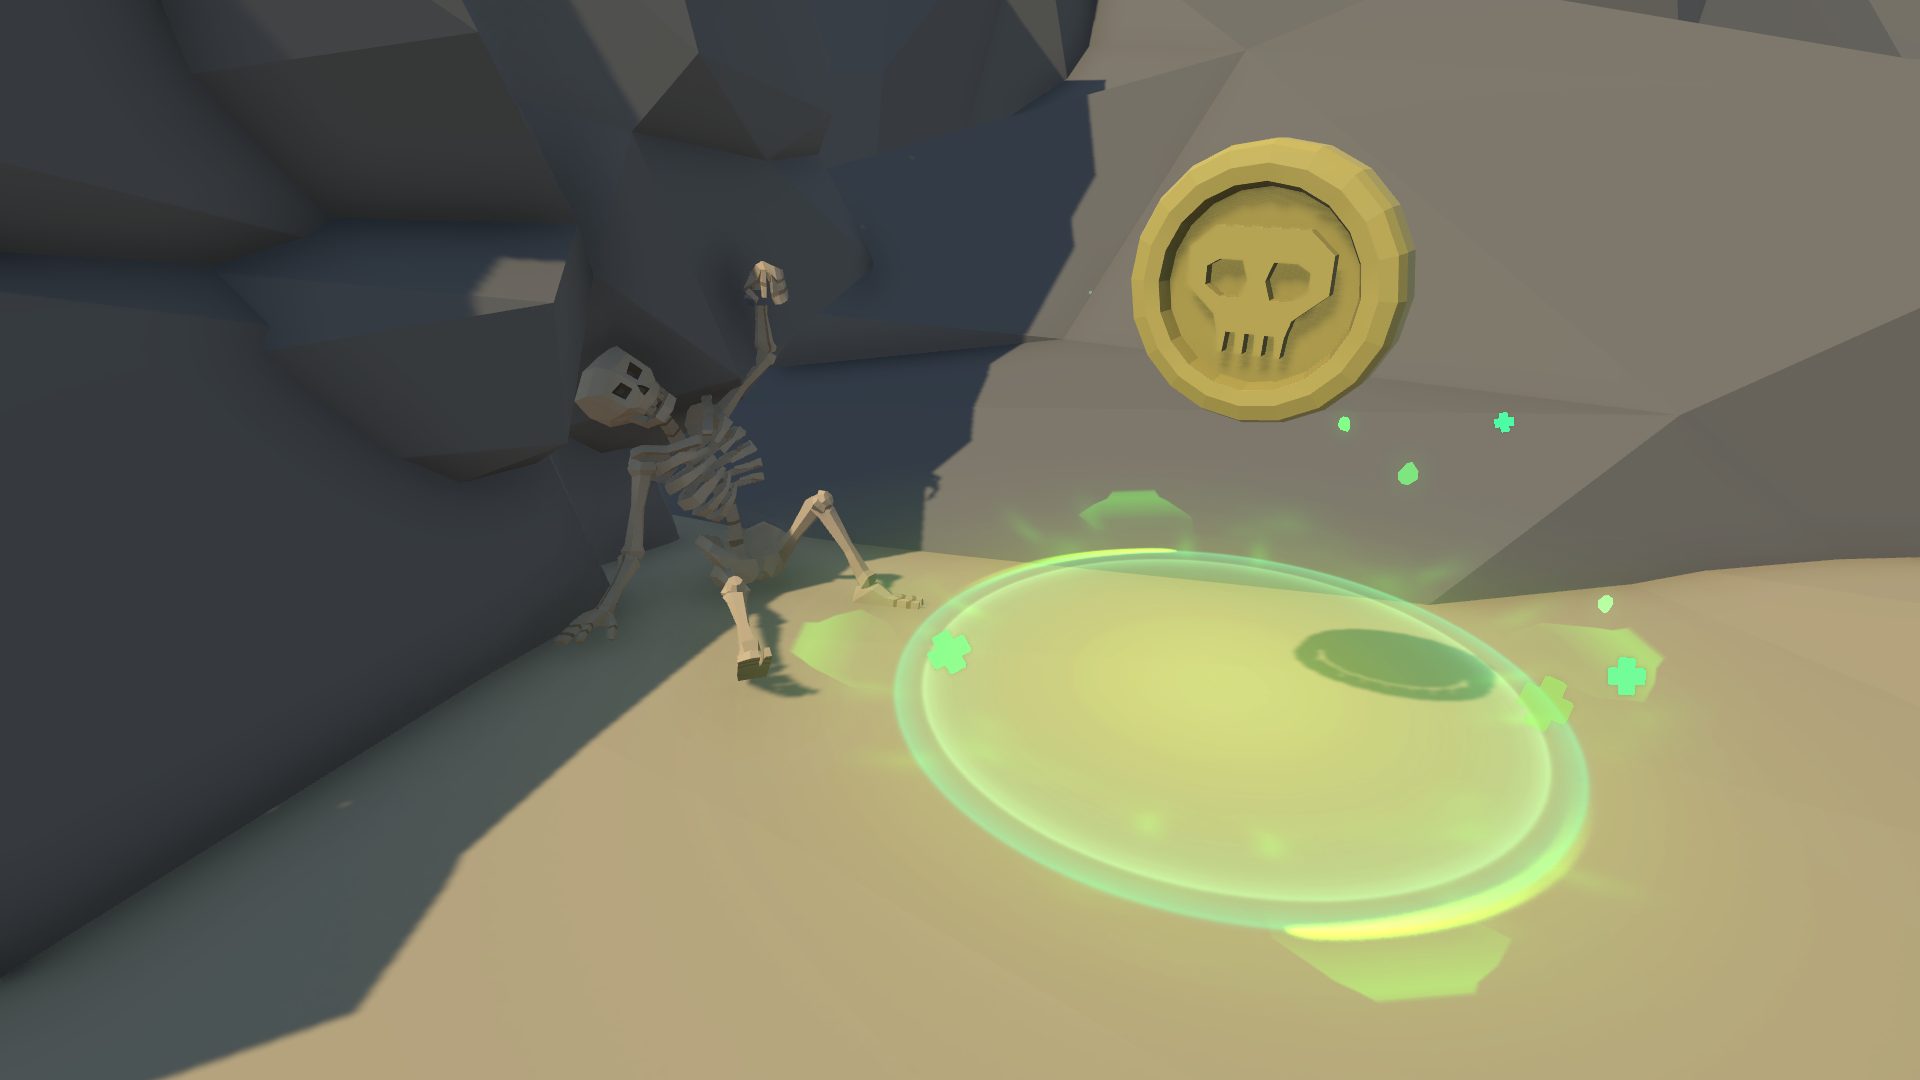
\includegraphics[width=.9\textwidth]{Figures/pickup.png}
	\caption{Zberateľný predmet minca}
	\label{pic:Pickup}
\end{figure}

Podobným spôsobom ako pri zberateľných predmetoch bola v projekte riešená aj interakcia s objektom Finish, ktorého úlohou je ukončiť hru v prípade, že s ním hráčov kontroler začne kolidovať. Taktiež teda obsahuje komponentu box collider nastavenú ako trigger a komponentu rigidbody. Pri štarte hry sa tento Finish rovnako ako zberateľné predmety zaregistruje pod objekt GameManager a v metóde \mbox{OnTriggerEnter()}, po overení, že naozaj koliduje s hráčom, vyvolá event \mbox{OnTriggered}. Nakoľko bol Finish využívaný aj v trénovacej fáze, bol pre tento účel vytvorený jednoduchý interface IFinish obsahujúci spomínanú metódu OnTriggered a jeho dve implementácie: FinishGame a FinshEpisode. Prvá spomínaná je využívaná v hlavnej scéne a ukončuje hru, druhá, ako názov napovedá, ukončuje trénovaciu epizódu v neprospech AI agenta. Jednotlivé trénovacie scenáre sú potom popísané v sekcií \ref{sec:Training}.

Po vyvolaní spomínaného eventu objekt GameManager overí prerekvizity výhry a pokiaľ ich hráč spĺňa ukončí hru. Tento postup je možné vidieť vo výpise \ref{src:FinishGame}. Pomocou eventu OnGameFinished zároveň všetkým odberateľom oznámi ukončenie hry. Najdôležitejší odberatelia eventu sú herná kamera a pohybový systém hráča, ktorí okamžite zastavia svoju činnosť a stanú sa pasívnymi. Zároveň s týmto sa hráčovi začne postupne zobrazovať informácia o úspešnom dokončení hry a po určitej dobe sa reštartuje scéna, čo umožní hráčovi skúsiť to znova napríklad s inými parametrami.

\vspace{8pt}
\begin{lstlisting}[label=src:FinishGame,caption={Ukončenie hry v prípade výhry hráča}]
private bool PrerequisitesMet()
{
    return (pickedBottles >= minBottles) && (pickedCoins >= minCoins);
}
private void GameFinished()
{
    if (!PrerequisitesMet())
    {
        ShowPrerequisitesNotMetInfo();
        return;
    }

    OnGameFinished?.Invoke();

    if (youWonUI != null)
        youWonUI.SetActive(true);

    StartCoroutine(RestartSceneCoroutine());
}
private IEnumerator RestartSceneCoroutine()
{
    yield return uiWait;
    SceneManager.LoadScene(SceneManager.GetActiveScene().name);
}
\end{lstlisting}

Medzi ďalšie kompetencie GameManagera patrí na základe nastavení uložených v objekte ConfigManager inštancovať pri štarte hry NPC agentov určeného typu na konkrétne pozície a rotácie. Bližší popis štruktúry agentov, ich inštancovanie a fungovanie je popísané v sekcií \ref{sec:Agents}.

Poslednou kompetenciou GameManagera je periodicky v rámci metódy OnUpdate() zisťovať od objektu InputManager, či bola stlačená klávesa na pozastavenie hry a na základe toho zobraziť hráčovi príslušný GUI element. Tento postup bol zvolený z dôvodu, že vstavaný input systém editoru Unity nedokáže spracovávať užívateľský vstup tzv. event-driven prístupom. Spomínaný GUI element je možné vidieť na obrázku \ref{pic:PauseUI} a umožňuje hráčovi rozhodnúť, či chce ukončiť hru alebo sa vrátiť do hlavnej ponuky. 

\begin{figure}[!htbp]
	\centering
	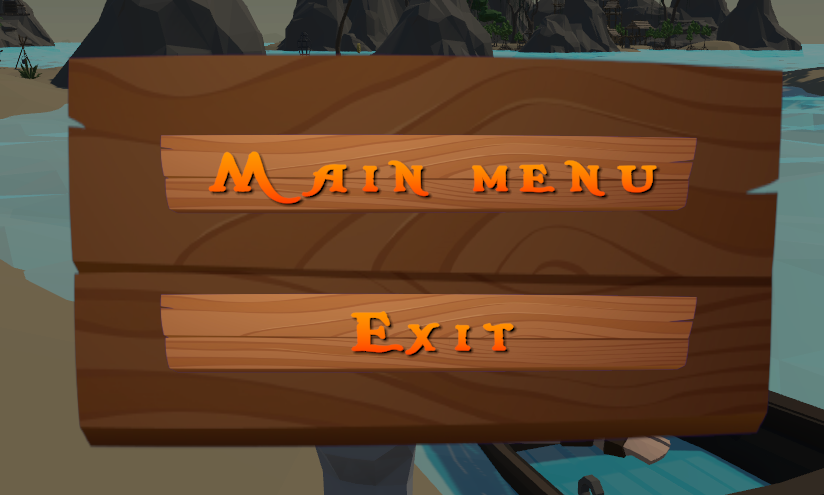
\includegraphics[width=.65\textwidth]{Figures/pauseUI.png}
	\caption{GUI element s umožňujúci návrat do hlavnej ponuky alebo ukončenia hry}
	\label{pic:PauseUI}
\end{figure}

Obe tlačidlá na GUI elemente zobrazenom na obrázku \ref{pic:PauseUI} obsahujú Unity komponentu Button, ktorá vie napríklad zmeniť farebnú schému elementu, keď nad ním hráč nadíde myšou. Dôležitejšou funkcionalitou je však možnosť priradiť eventu OnClick ľubovoľný objekt priamo v editore a interakcia s tlačidlom dokáže zavolať na tomto objekte určenú verejnú metódu, čo demonštruje obrázok \ref{pic:OnClick}. 

\begin{figure}[!htbp]
	\centering
	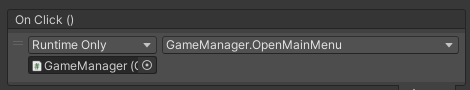
\includegraphics[width=.8\textwidth]{Figures/OnClick.png}
	\caption{Nastavenie OnClick eventu tlačidla v editore}
	\label{pic:OnClick}
\end{figure}

V tomto prípade bol tlačidlám predaný objekt GameManager a volané boli jeho dve verejné metódy OpenMainMenu() a QuitGame() zobrazené vo výpise \ref{src:MMQuit}.

\vspace{8pt}
\begin{lstlisting}[label=src:MMQuit,caption={Metódy na návrat do hlavnej ponuky a ukončenie hry}]
public void OpenMainMenu()
{
    SceneManager.LoadScene(0);
}
public void QuitGame()
{
#if UNITY_EDITOR
    UnityEditor.EditorApplication.isPlaying = false;
#endif
    Application.Quit();
}
\end{lstlisting}

Metóda OpenMainMenu() načíta scénu s build indexom 0. Tento postup je vhodné aplikovať, keď máme fixne dané poradie scén v zostavení aplikácie. Zamedzí sa tým zbytočnému prehľadávaniu scén podľa mena. Poradie scén v rámci tohto projektu bolo popísané v sekcií \ref{sec:GameStructure}. 

Ukončenie hry potom prebieha jednoduchým zavolaním metódy Application.Quit(). Tento prístup však nefunguje na aplikáciu spustenú v editore Unity. Z tohto dôvodu je v rámci direktivy preprocesoru UNITY\_EDITOR, nutné aj nastavenie premennej isPlaying v triede UnityEditor.EditorApplication na hodnotu false. 

Direktívy preprocesoru v jazyku C\# umožňujú selektívne zahrnúť alebo vylúčiť kód z kompilácie na základe toho, či sú alebo nie sú definované určité skriptovacie symboly. Editor Unity ná na tieto účely preddefinované symboly umožňujúce rozlíšiť rôzne platformy či práve zostavenie aplikácie od behu v editore \cite{ConditionalCompilation}.

\section{Hlavná ponuka hry}
\label{sec:MainMenuAndUI}

Ako už bolo spomenuté v predchádzajúcich sekciách vytvorená hra obsahuje scénu s hlavnou ponukou. Táto scéna obsahuje informačnú tabuľu s aktuálnymi nastaveniami a štyri aktívne prvky užívateľského rozhrania. Ide o tlačidlá Play, Options, Credits a Exit. Tieto tlačidlá opäť obsahujú Unity komponentu Button a referenciu na objekt, ktorého verejné metódy volajú. Hlavnú ponuku je možné vidieť na obrázku \ref{pic:MainMenu}.

\begin{figure}[!htbp]
	\centering
	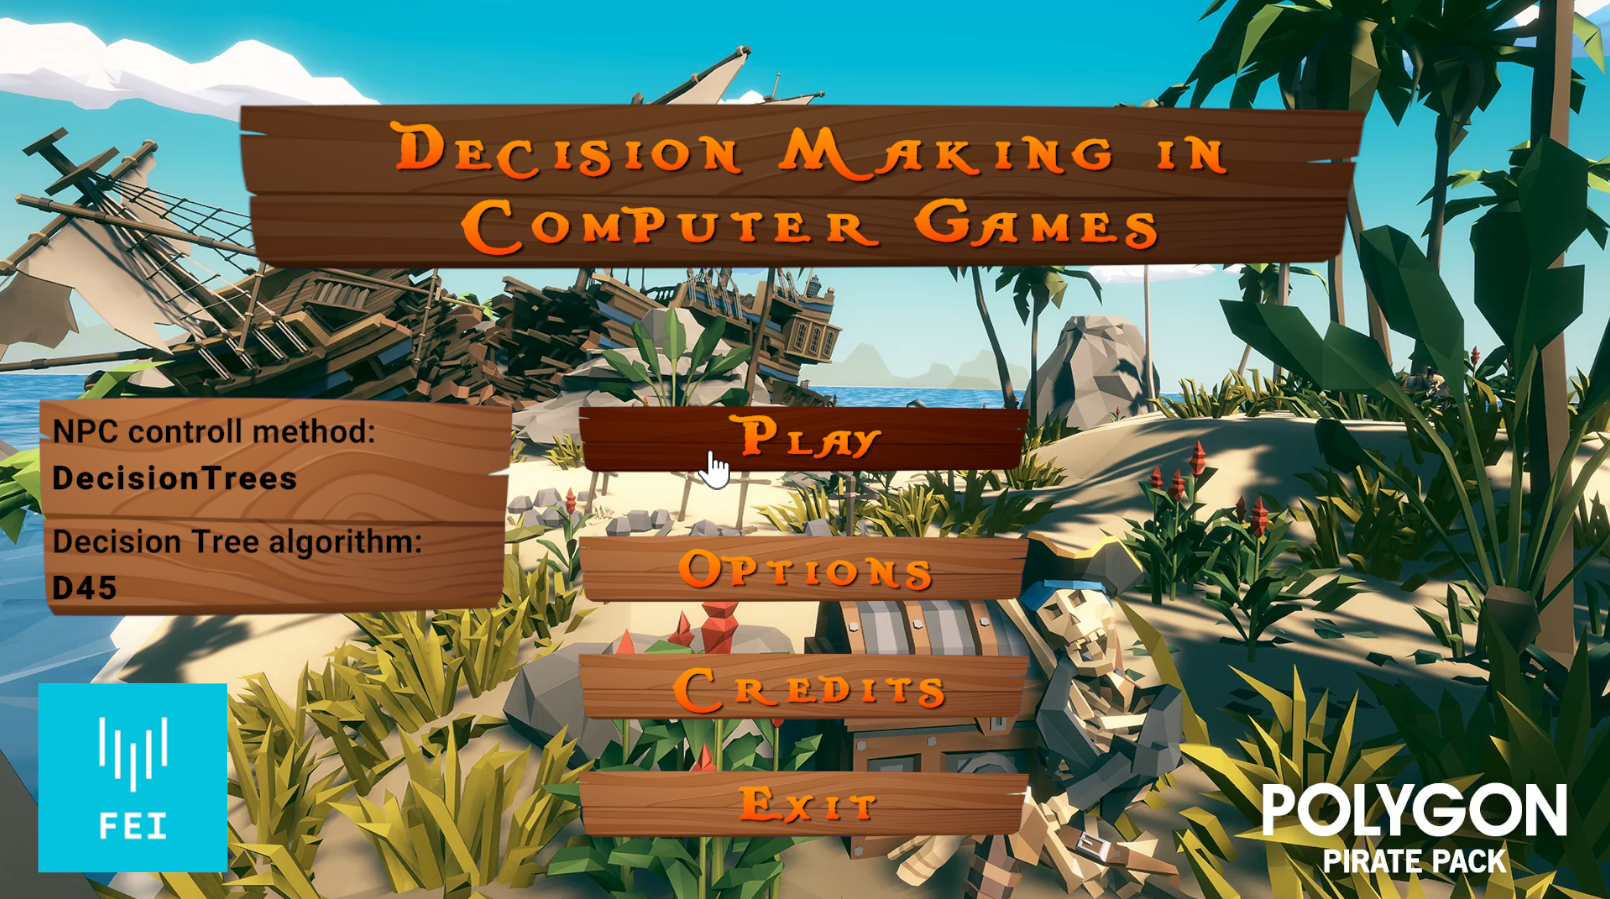
\includegraphics[width=.9\textwidth]{Figures/mainMenu.png}
	\caption{Hlavná ponuka hry}
	\label{pic:MainMenu}
\end{figure}

Informačná tabuľa na ľavej strane obrazovky zobrazuje, či budú NPC agenti v hre ovládaní rozhodovacím stromom alebo pomocou spätnoväzobného učenia. Pokiaľ budú agenti ovládaní pomocou rozhodovacieho stromu v spodnej časti tabule sa zobrazí aj algoritmus, ktorým má byť strom zostrojený. Tieto nastavenia sú perzistentné a teda ostanú uchované aj po vypnutí aplikácie. Zmeny je možné vykonať v ponuke Options. Stlačenie príslušného tlačidla v tejto ponuke vyvolá zmenu na objekte ConfigManager. Ten pomocou jednoduchej metódy Serialize() tieto zmeny aktualizuje na disku v súbore \textit{settings.txt} uloženom v adresári danom premennou \textit{Application.persistentDataPath}. Konkrétna cesta sa líši v závislosti od aktuálnej platformy. Zároveň je zmena v dátach propagovaná pomocou eventu OnDataChanged, ktorého odberateľom je hlavná ponuka, ktorá tieto zmeny aktualizuje v informačnej tabuli.

Tlačidlo Exit ukončí beh aplikácie a tlačidlo Play spustí hlavnú scénu hry. Obdobná funkcionalita bola demonštrovaná už vo výpise \ref{src:MMQuit}.

Tlačidlo Credits zavolá metódu SetActive() so vstupným parametrom nastaveným na false na svojom predkovi, ktorý združuje všetky tlačidlá, informačnú tabuľu a tabuľu s menom aktuálnej ponuky. Zároveň obdobným spôsobom aktivuje ponuku Credits, ktorá mu bola referencovaná v editore. 

Tlačidlo Options potom využíva rovnaký prístup na zobrazenie ponuky s výberom typu NPC agenta proti ktorému chce hráč hrať. V prípade, že hráč vyberie možnosť Decision Trees je mu ešte zobrazená ponuka s výberom algoritmu, ktorý chce použiť na zostavenie rozhodovacieho stromu.

Každá vnorená ponuka, ktorá sa stane aktívna sa začne periodicky dopytovať objektu InputManager, či bola stlačená príslušná klávesa na návrat do predchádzajúcej ponuky. Na tento účel bola vytvorená jednoduchá trieda zobrazená vo výpise \ref{src:SubMenu}.

\vspace{8pt}
\begin{lstlisting}[label=src:SubMenu,caption={Trieda SubMenu}]
public class SubMenu : MonoBehaviour
{
    [SerializeField]
    private GameObject currentSubMenu;
    [SerializeField]
    private GameObject previousSubMenu;

    private void Update()
    {
        if (MainManager.Instance.InputManager.WasCancelledLastFrame)
        {
            currentSubMenu.SetActive(false);
            previousSubMenu.SetActive(true);
        }
    }
}
\end{lstlisting}

Jednotlivé ponuky sú v triede referencované pomocou atribútu \textit{SerializeField} a na jednotlivých objektoch boli nastavené ručne v editore. Atribút \textit{SerializeField} vynúti serializáciu u neverejných členských premenných \cite{SerializeField}, čím sa neporušuje princíp zapuzdrenia a zároveň to umožňuje jednoducho referencovať medzi sebou objekty priamo v editore Unity pomocou tzv. Drag \& Drop či výberu z rolovacej ponuky. Nie je teda nutné prehľadávať objekty v scéne alebo riešiť prístup k danému objektu architektonicky na úrovni kódu. Tento prístup však nie je možné použiť na prepojenie dvoch objektov, pričom jeden z nich je prítomný v scéne od začiatku a druhý je inštancovaný za behu aplikácie. Všetky jednotlivé ponuky sú súčasťou hierarchie scény od jej spustenia, takže nebol s týmto prístupom problém. Diagram všetkých ponúk je možné vidieť na obrázku \ref{pic:MainMenuScheme}.

\begin{figure}[!htbp]
	\centering
	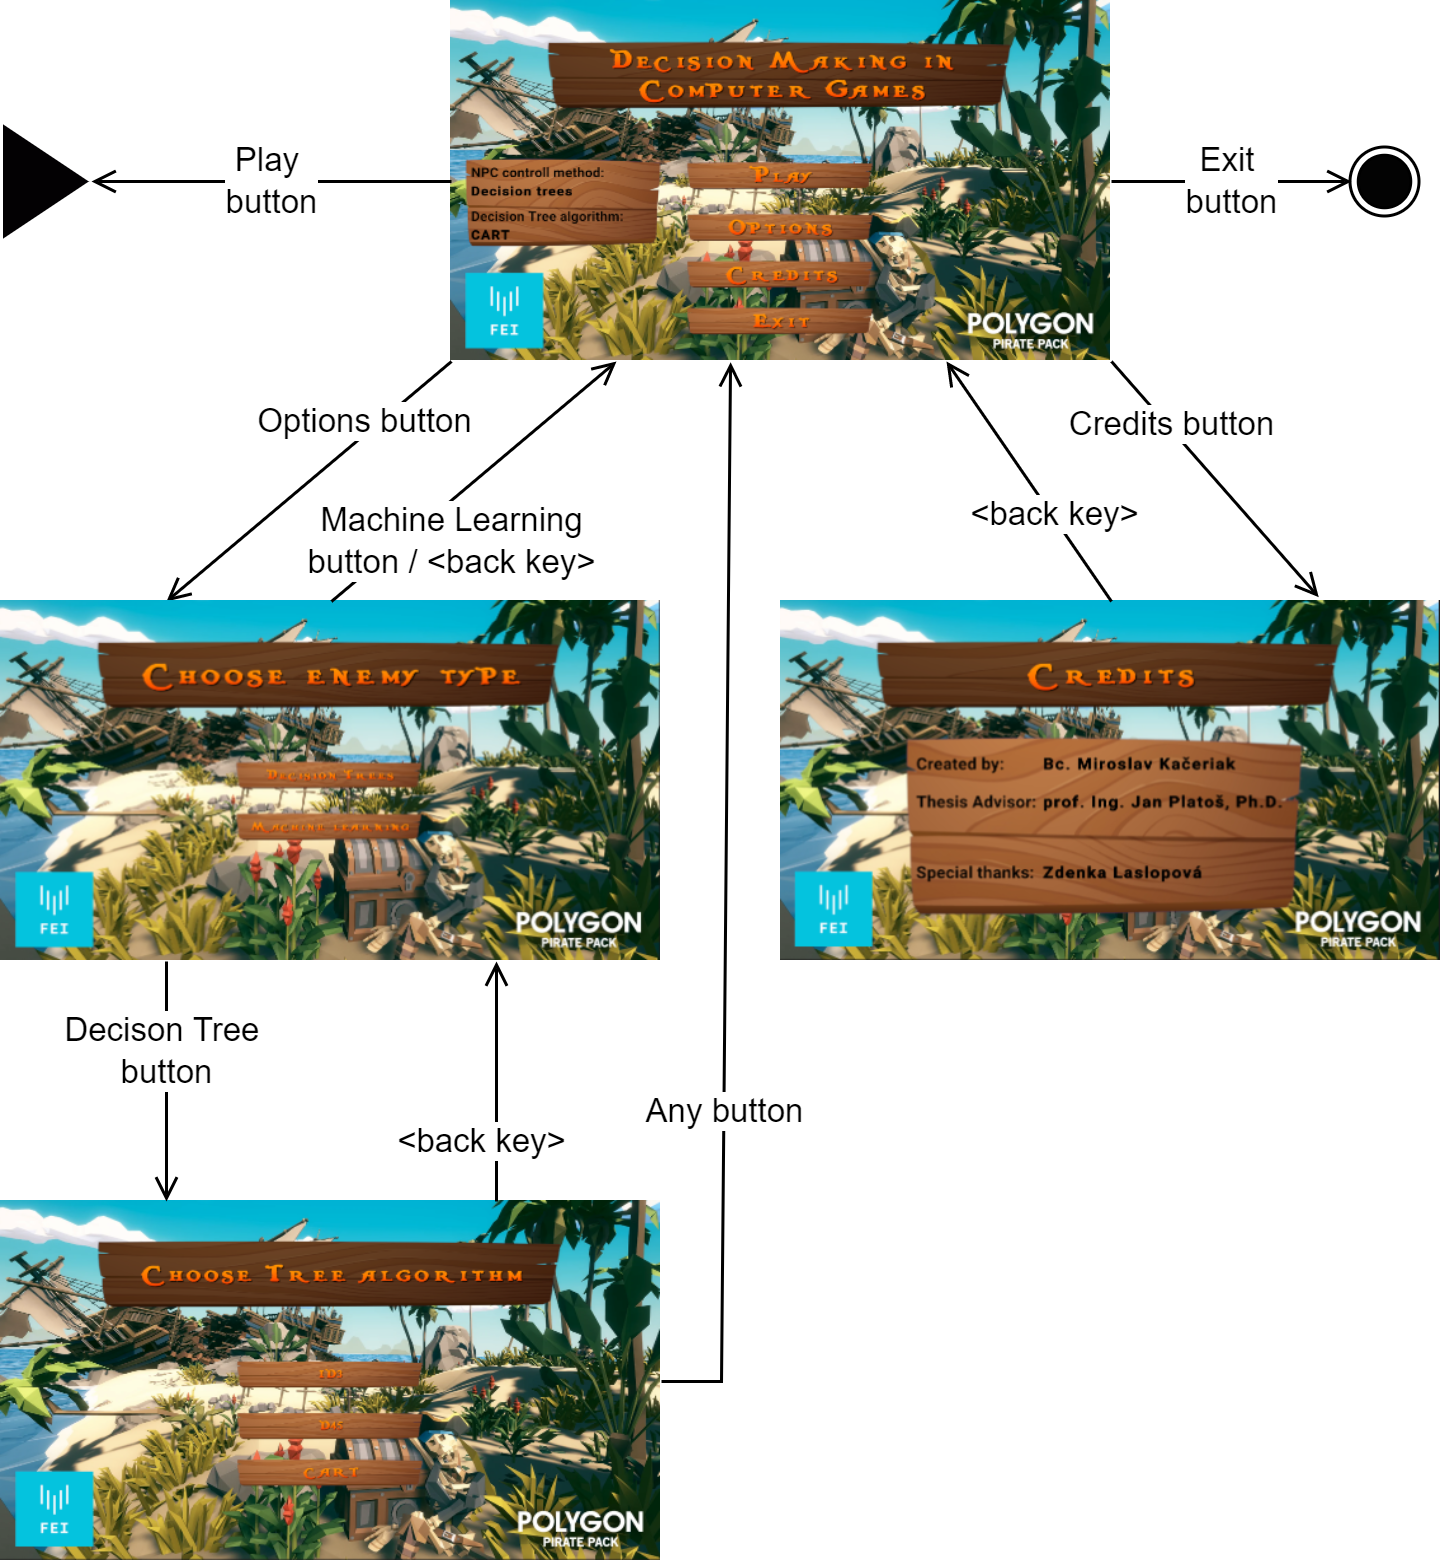
\includegraphics[width=.85\textwidth]{Figures/mainMenuScheme.png}
	\caption{Diagram obrazoviek hlavnej ponuky}
	\label{pic:MainMenuScheme}
\end{figure}

% Chapter 5
\chapter{Architektúra hráčskej postavy}
\label{sec:Player}
Jednou z najdôležitejších súčasti hier ovládaných z pohľadu tretej osoby je práve hráčska postava. Tá reaguje na hráčov vstup zmenou smeru alebo rýchlosti pohybu, akciami ako skok, útok, úhyb či kontextuálnou interakciou s nejakým objektom v hre a podobne. Na postavu hráča pôsobí určitá forma gravitácie a s tým súvisiaca kolízia s hernou plochou a ostatnými statickými či dynamickými objektami. Hráčska postava má spravidla nastavenú nejakú hodnotu zdravia či života, ktorá sa v čase mení napríklad po páde z veľkej výšky či po zásahu od nepriateľa. Hodnota ostávajúceho zdravia je často hráčovi prezentovaná vo forme GUI ukazovateľa. 

Táto kapitola popisuje akým spôsobom bolo k jednotlivým problémom pristupované v tomto projekte. Niektoré princípy je možné s väčšími či menšími úpravami aplikovať obecne, iné sú poplatné editoru Unity. 

\section{Prehľad komponentov}
\label{sec:PlayerComponentOverview} 
Samotný objekt hráčskej postavy sa skladá z dvoch objektov, ktoré sa zvyknú nazývať kontroler a model. 

Model reprezentuje vizuálnu stránku objektu, teda postavu samotnú a ďalšie menšie objekty, ktoré má táto postava na sebe. Pri zložitejších modeloch ide o hierarchiu čítajúcu stovky objektov reprezentujúce jednotlivé časti tela. V tomto prípade je využitý tzv. low poly model, ktorý je vcelku a pod sebou má iba zopár vizuálnych doplnkov, ktoré postava nosí okolo pása.

Kontroler, na druhú stranu obsahuje sadu komponentov, ktoré obstarávajú pohyb, gravitáciu, kolíziu a ľubovoľnú ďalšiu funkcionalitu. Dôležitou komponentou kontrolera je práve Unity komponenta Character Controller. Na nej je možné nastaviť rôzne parametre definujúce tvar kolíznej kapsule, maximálnu výšku kroku, ktorý môže postava vykonať bez nutnosti vyskočiť apod. Túto kapsulu s kompletnou vizuálnou stránkou hráča je možné vidieť na obrázku \ref{pic:PlayerController}.

\begin{figure}[!htbp]
	\centering
	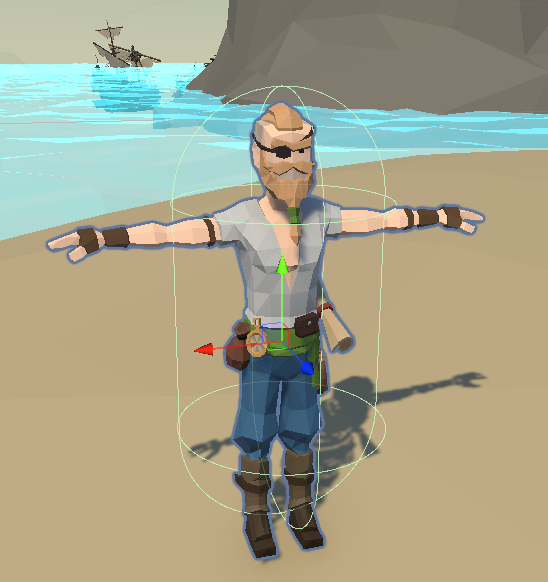
\includegraphics[width=0.54\textwidth]{Figures/controller.png}
	\caption{Hráčka postava s komponentou Character Controller}
	\label{pic:PlayerController}
\end{figure}

Na objekte kontroler sa ďalej nachádzajú komponenty PlayerBrain, PlayerBody, PlayerMovement, PlayerAutomaticMovement a NavMeshAgent. Posledné dve spomenuté komponenty sú v predvolenom stave deaktivované a aktivuje ich komponenta PlayerBrain v prípade, že má objekt ConfigManager v editore nastavenú premennú PlayerControll na hodnotu Automatic. Toto je využívané primárne v trénovacích scenároch, ktoré sú bližšie popísané v sekcií \ref{sec:Training}. V tomto prípade taktiež komponenta PlayerBrain vypne komponentu PlayerMovement, čím znemožní ovládať hráča pomocou vstupu z periférií. 

Poslednou kompetenciou komponenty PlayerBrain je držať referencie na zvyšné komponenty a inicializovať ich. Počas inicializačnej fázy sú jednotlivým komponentám predané referencie na iné komponenty ktoré potrebujú pre svoje fungovanie. Tento prístup umožňuje centrálne riadiť prepojenia medzi komponentami bez nutnosti ich rôzne referencovať navzájom v editore.

\section{Prijímanie poškodenia}
\label{sec:DealingDamage}
Hráčska postava je zraniteľná voči útoku nepriateľského NPC agenta. Maximálna hodnota poškodenia, ktorú hráčska postava môže inkasovať kým zomrie je nastavená v komponente PlayerBody. Táto komponenta teda obsahuje maximálnu hodnotu zdravia, ktorá sa hráčovi nastaví na začiatku hry a aktuálnu hodnotu zdravia, ktorá klesá s prijímaným poškodením. Všetká potrebná funkcionalita súvisiaca s prijímaním poškodenia vrátane propagovania informácie o zmene hodnoty zdravia či smrti danej postavy bola zjednotená pod rozhranie IDamageable. Toto rozhranie okrem komponenty PlayerBody implementuje aj abstraktná komponenta NPCBody, ktorá bude bližšie popísaná v sekcií \ref{sec:Agents}. Spomínané rozhranie je možné vidieť vo výpise \ref{src:IDamageable}. 

\vspace{8pt}
\begin{lstlisting}[label=src:IDamageable,caption={Rohranie IDamageable}]
public interface IDamageable
{
    public float MaxHealth { get; }
    public float Health { get; }

    public event Action<float> OnHealthChanged;
    public event Action OnDied;

    public void DealDamage(float damage);
}
\end{lstlisting}

Komponenta PlayerBody sa pri spustení hry zaregistruje pod objekt GameManager ako implementácia rozhrania IDamageable. GameManager sa v tomto momente stane odberateľom eventu OnHealthChanged za účelom aktualizácie GUI elementu zobrazujúceho aktuálny stav zdravia hráčskej postavy. Tento element sa zvykne nazývať Health bar.

Zavolanie metódy DealDamage() na hráčskej postave teda spôsobí odrátanie hodnoty poškodenia od aktuálnej hodnoty zdravia a vyvolanie spomínaného eventu. Pokiaľ táto hodnota zdravia klesne na nulu je na hráčskej postave deaktivované ovládanie pohybu a vyvolá sa event OnDied. Na tento event zareaguje odberateľ GameManager, ktorý vyvolá event OnGameEnded, na základe ktorého sa deaktivuje ovládanie kamery a následne je hráčovi zobrazená informácia o konci hry. Po určitom čase je scéna reštartovaná a hráč to môže skúsiť znova a lepšie. 

Informáciu o konci hry spolu s prázdnym GUI elementom Health bar je možné vidieť na obrázku \ref{pic:YouDied}. Na tomto obrázku je možné povšimnúť si aj GUI elementy zobrazujúce hráčovi počet nazbieraných predmetov spolu s minimálnym počtom, ktorý je vyžadovaný na úspešné dokončenie hry. Aktualizácia počtu zozbieraných predmetov v GUI záležitosťou nastavenia reťazca v premennej text príslušného objektu. 

\begin{figure}[!htbp]
	\centering
	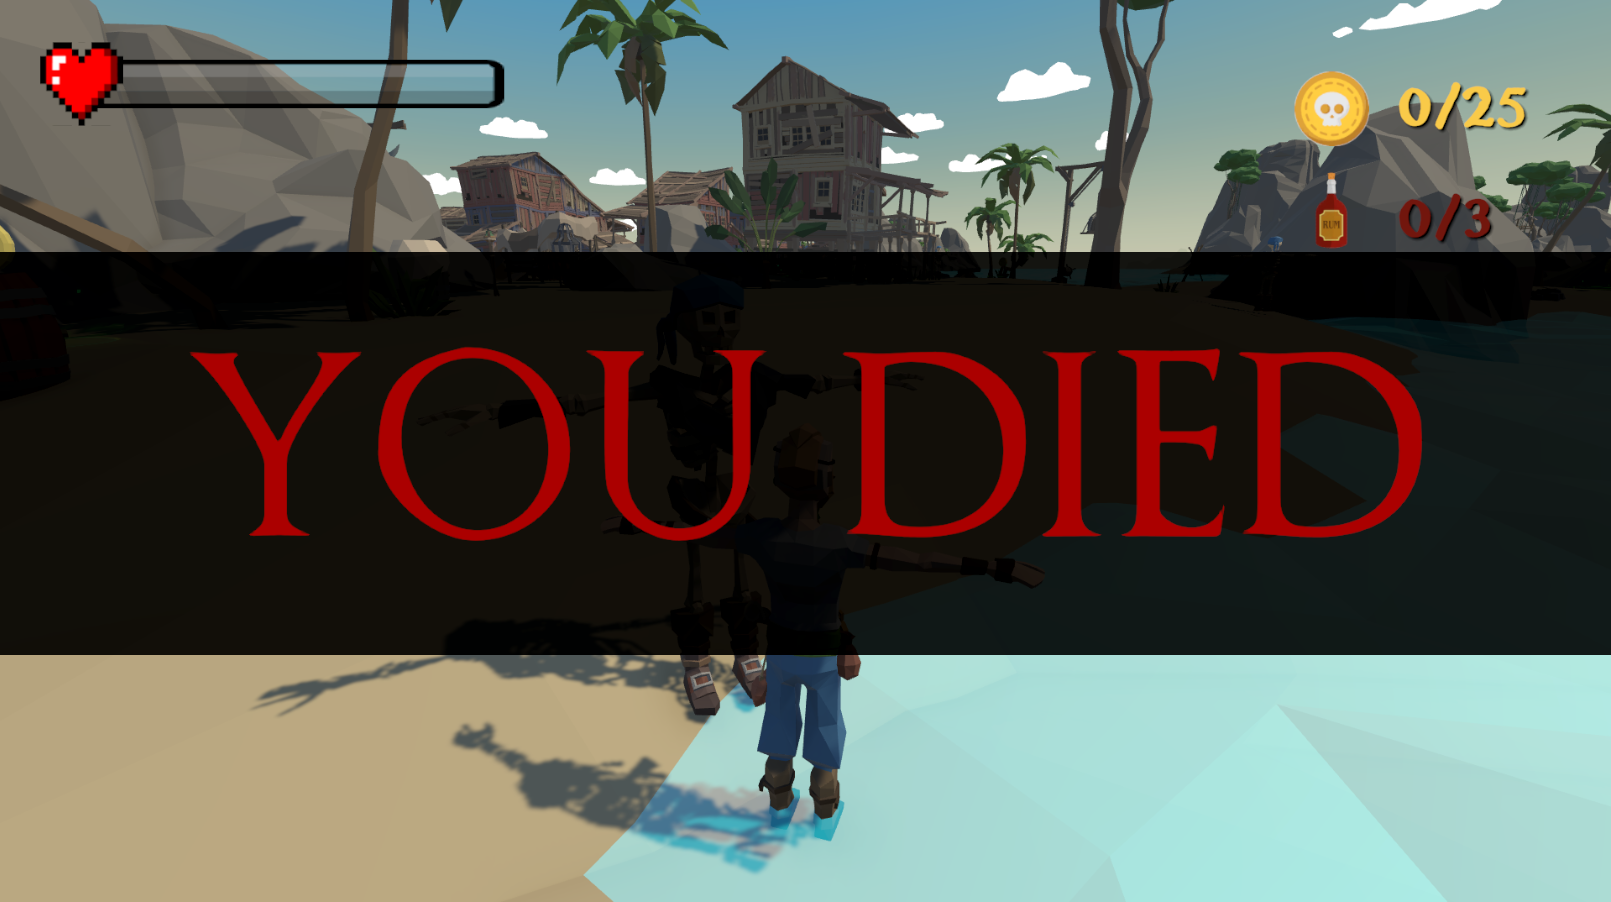
\includegraphics[width=.8\textwidth]{Figures/youDied.png}
	\caption{GUI elementy v hlavnej scéne}
	\label{pic:YouDied}
\end{figure}

GUI element Health bar sa skladá z troch častí: výplň, obrys a ikona srdca. Na aktualizáciu hodnoty v tomto GUI elemente je využívaná Unity komponenta Slider. Táto komponenta má množstvo nastavení a parametrov vrátane objektu, ktorého rozmery bude Slider ovplyvňovať (v tomto prípade výplň elementu) a maximálnej hodnoty. Tá sa pri spustení hry nastaví na hodnotu maximálneho zdravia hráčskej postavy a je teda možné priamo bez prepočtu nastavovať hodnotu Slideru v reakcii na zmenu zdravia hráča.

\section{Pohyb}
\label{sec:PlayerMovement} 
Jednou z najdôležitejších súčastí hráčskej postavy je práve možnosť jej ovládania pomocou periférií. Pre tento účel bola vytvorená komponenta PlayerMovement. Táto komponenta teda periodicky obstaráva komunikáciu s objektom InputManager a komponentou Character Controller a získané vstupy transformuje na pohyb postavy v trojrozmernom hernom priestore.

Existuje množstvo prístupov k tejto problematike a v závislosti od typu hry či členitosti herného prostredia môže byť práve pohyb hráča veľmi komplexnou témou hlavne v kombinácií s realistickými animáciami.

V tomto projekte bol využitý základný systém využívajúci možností vstavanej Unity komponenty Character Controller a to ako na pohyb tak aj na zisťovanie, či sa hráč nachádza na pevnej zemi. Hráčovi je okrem základného pohybu do rôznych smerov umožnené skákať, či spomaliť svoj pohyb, čím sa zníži rozsah šírenia zvuku jeho krokov. Pohyb hráča taktiež podlieha základnej simulácií gravitácie. Metódu Update() komponenty PlayerMovement, ktorá obstaráva vyššie popísanú funkcionalitu je možné vidieť vo výpise \ref{src:PlayerMovement}.

\vspace{8pt}
\begin{lstlisting}[label=src:PlayerMovement,caption={Metódy komponenty PlayerMovement obstarávajúce pohyb hráčskej postavy}]
void Update()
{
    var currentSpeed = speed;

    if (controller.isGrounded)
        UpdateGrounded(ref currentSpeed);

    Vector3 direction = new Vector3(horizontal, 0, vertical);
    float magnitude = Mathf.Clamp01(direction.magnitude) * currentSpeed;
    direction.Normalize();

    float angle = SmoothAngleFromDirection(direction);
    if (direction != Vector3.zero)
        transform.localRotation = Quaternion.Euler(0f, angle, 0f);

    Vector3 moveDirection = Quaternion.Euler(0f, angle, 0f) * Vector3.forward;
    Vector3 velocity = moveDirection.normalized * magnitude;

    ySpeed += Physics.gravity.y * Time.deltaTime;
    velocity.y = ySpeed;

    controller.Move(velocity * Time.deltaTime);
    MakeNoise(velocity);
}
private void UpdateGrounded(ref float currentSpeed)
{
    ySpeed = defaultYSpeed;

    horizontal = inputManager.Horizontal;
    vertical = inputManager.Vertical;

    if (inputManager.WasJumpingThisFrame)
        ySpeed = jumpSpeed;

    if (inputManager.IsCrounching)
        currentSpeed /= 2;
}
\end{lstlisting}

Vo výpise \ref{src:PlayerMovement} je možné si povšimnúť, že pokiaľ sa hráčska postava nachádza na zemi, je možné zmeniť jej smer na osách X a Z, vyskočiť, či znížiť rýchlosť pohybu na polovicu, čo sa prejaví pri šírení zvuku krokov. V tomto prípade je aj vyresetovaná rýchlosť postavy na ose Y a to na 0, prípadné na malé záporné desatinné číslo. V momente kedy hráč stlačí tlačidlo skoku, je táto rýchlosť nastavená na hodnotu výšky skoku a počas nasledujúcich snímkov bude klesať rýchlosťou danou hodnotou gravitačnej konštanty vynásobenej časom medzi jednotlivými snímkami. Keď postava dopadne na zem je táto rýchlosť opäť vyresetovaná a medzi jednotlivými snímkami sa mení len minimálne v závislosti na hodnote FPS a teda mierne tlačí postavu k zemi, čím sa eliminujú problémy s prípadnou zlou detekciu zeme pri nerovnom teréne.

Následne sa na základe hráčskeho vstupu vypočíta smer a rýchlosť pohybu, ktorým sa má postava vydať a výsledná hodnota, opäť vynásobená časom medzi jednotlivými snímkami, je odoslaná do metódy Move() komponenty Character Controller. Táto metóda vykoná pohyb postavy, pokiaľ to kolízna kapsula či výška nerovného terénu dovolí. Násobenie hodnotou Time.deltaTime, teda časom medzi jednotlivými snímkami spôsobí, že rýchlosť pohybu bude nezávislá od snímkovej frekvencie hry.

Taktiež je vhodné neaplikovať smer na rotáciu postavy priamo, ale vziať do úvahy aktuálnu rotáciu kamery, teda smer, do ktorého sa hráč pozerá. Z dôvodu eliminácie instantnej zmeny rotácie, čo spôsobí nepríjemný efekt teleportácie modelu do daného smeru je tiež vhodné robiť veľké zmeny postupne. Tento prístup je znázornený vo výpise \ref{src:SmoothAngleFromDirection}.

\vspace{8pt}
\begin{lstlisting}[label=src:SmoothAngleFromDirection,caption={Postupná zmena rotácie postavy v súlade s rotáciu kamery}]
private float SmoothAngleFromDirection(Vector3 direction)
{
    var cameraY = (cameraTransform == null) ? 
    cameraTransform.eulerAngles.y : 0.0f;

    float tempAngle = Mathf.Atan2(direction.x, direction.z) * Mathf.Rad2Deg + cameraY;
    return Mathf.SmoothDampAngle(transform.eulerAngles.y, tempAngle, ref turnSmoothVelocity, turnSmoothTime);
}
\end{lstlisting}

Poslednou kompetenciou komponenty PlayerMovement je vydávanie zvuku pri pohybe. To je realizované pomocou metódy MakeNoise() vo výpise \ref{src:PlayerMovement}. Táto metóda na základe vstupného parametru, ktorý reprezentuje rýchlosť pohybu vypočíta druhú mocninu dĺžky X a Z zložky vstupného vektoru. Tú spolu s aktuálnou pozíciou vloží ako parametre koštruktora readOnly štruktúry Noise a následne zavolá na objekte SoundManager metódu MakeNoise, ktorej danú inštanciu štruktúry odošle ako parameter. Tento postup sa vykonáva v pravidelných intervaloch, ktorých dĺžka je daná konštantou stepDelay a za splnenia podmienky, že hráč nie je statický. 

SoundManager následne vytvorí tzv. SphereCast a teda získa všetky kolidery v rádiuse daného bodu v priestore. Všetky nájdené objekty sú skontrolované na prítomnosť komponenty Hearing. Ak objekt obsahuje túto komponentu je na nej zavolaná metóda RespondToNoise(), ktorej je predaná pozícia danej inštancie zvuku. Reakcia na tento podnet je bližšie popísaná v sekcií \ref{sec:Perception}. Pomocou Unity metódy OnDrawGizmosSelected() bola taktiež v editore vytvorená jednoduchá vizualizácia zvuku za účelom ladenia

\section{Kamera}
\label{sec:Camera}

Kamera je veľmi dôležitým prvkom každej hry. Nielenže hráč pomocou nej môže sledovať dianie v hernom svete ale už samotným pohybom tejto kamery môže ovplyvňovať napríklad smer pohybu hráčskej postavy, čo bolo demonštrované v predchádzajúcej sekcií. 

V editore Unity je možné využiť na snímanie diania v hre predpripravenú komponentu Camera. Tá umožňuje nastavenie rôznych parametrov od FOV, typu projekcie, vzdialenosti orezávacích rovín až po napríklad anti-aliasing. Bez prítomnosti kamery v scéne je renderovaná iba čierna obrazovka s varovným nápisom a GUI. Kamier v scéne môže byť niekoľko a je možné medzi nimi plynulo prepínať napríklad v rámci filmových sekvencií čí mierenia so zbraňou.

Ovládanie kamery bolo realizované pomocou modulu Cinemachine od spločonosťou Unity, ktorá vytvára samotný editor. Tento modul je zdarma dostupný z oficiálneho repozitára a obsahuje niekoľko typov kamier, ktoré je možné použiť. V tomto projekte je využitá tzv. Free Look Camera. Po výbere kamery je na objekt obsahujúci Unity komponentu Camera pridaná komponenta z tohto modulu s názvom CinemachineBrain a následne je vytvorený nový herný objekt, ktorý obsahuje komponentu s názvom odpovedajúcim vybranému typu kamery. Komponenta CinemachineBrain sa prepojí s komponentou tohto nového objektu, a ten prevezme kontrolu nad pozíciou a rotáciou pôvodnej kamery bez nutnosti ručného nastavovania týchto parametrov zo skriptu.

\begin{figure}[!htbp]
	\centering
	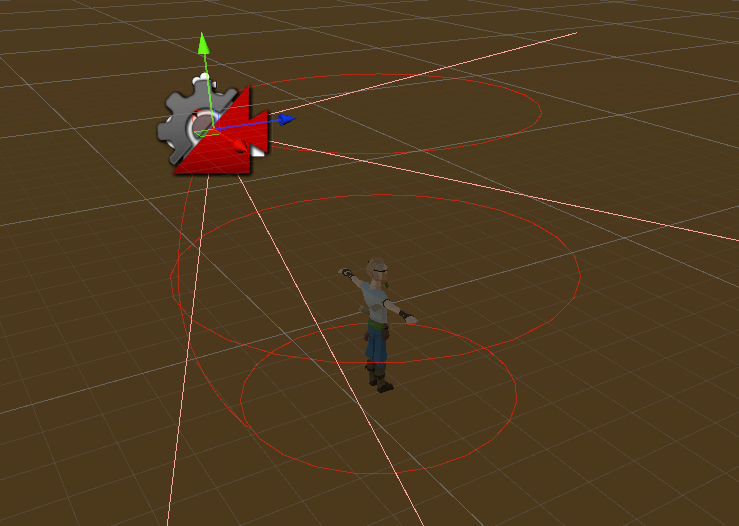
\includegraphics[width=.7\textwidth]{Figures/obruce.png}
	\caption{Vizualizácia obručí, po ktorých sa pohybuje herná kamera}
	\label{pic:Cinemachine}
\end{figure}

Komponenta ovládajúca kameru má veľké množstvo nastavení, ktorých popis by presahoval rámec tejto práce. Dôležitým parametrami sú hlavne referencie na objekt, ktorý má kamera prenasledovať a na ktorý sa má zamerať. V tomto prípade bola na oba prípady použitá referencia hráčskej postavy. Ďalej boli na tomto mieste nastavené rýchlosti či rozsah pohybu kamery na jednotlivých osách, ktoré boli zároveň namapované na príslušné osy vstupných periférií. Kvôli kolízií kamery s hernými objektami bola ešte pridaná a nastavená komponenta Cinemachine Collider.

Samotná kamera sa potom pohybuje po troch obručiach - spodnej, strednej a hornej. Výšku a priemer týchto obručí je taktiež možné upraviť a každá z nich má separátne nastavenia, ktoré určujú stred pohľadu kamery, mŕtvu zónu, rýchlosť s akou sa kamera snaží dohnať svoj cieľ apod. Tieto obruče sú pre lepšiu predstavu znázornené na obrázku \ref{pic:Cinemachine}.

%Chapter 6
\chapter{Architektúra NPC agentov}
\label{sec:Agents}
Ako už bolo spomenuté v predchádzajúcich kapitolách, projekt obsahuje dva typy NPC agentov. Prvý typ sa rozhoduje na základe rozhodovacieho stromu zostrojeného zo vstupných dát a druhý typ agentov využíva na rozhodovanie model natrénovaný pomocou spätnoväzobného učenia. Jednotlivé typy NPC sa líšia aj v prístupe k navigácií priestorom či kolízií a ďalšími detailami v skladbe či funkcionalite jednotlivých komponentov. Táto kapitola si kladie za cieľ popísať štruktúru jednotlivých typov NPC, ich spoločné vlastnosti a odlišnosti s dôrazom na percepciu, teda zmyslové vnímanie jednotlivých NPC agentov.

\section{Spoločné prvky oboch typov agentov}
\label{sec:AgentsBoth}

Prvým spoločným prvkom NPC agentov je okrem iného aj ich inštancovanie. Túto funkcionalitu obstaráva objekt EnemySpawner nachádzajúci sa v scéne. Potomkami tohto objektu v hierarchií sú prázdne objekty, tzv. spawn pointy, ktoré sú ručne rozmiestnené po hernej ploche. V momente spustenia scény sú získané Transform komponenty týchto objektov, ktoré združujú pozíciu, rotáciu a mierku objektu. Tie potom pri procese inštancovania zabezpečujú, že objekt bude inštancovaný na určenú pozíciu v hernom svete a s určenou rotáciou. Pri tomto procese je ešte nutná referencia na tzv. prefab herného objektu a voliteľným prvkom je objekt, ktorý sa stane rodičom novo inštancovaných objektov. 

Prefab v editore Unity je možné chápať ako šablónu herného objektu spolu s jeho komponentami, nastavenými hodnotami a podradenými hernými objektami. Túto šablónu je možné opakovane použiť v rámci jednej scény ale aj vo viacerých scénach. Tento systém ponúka efektívny spôsob správy herných objektov a synchronizáciu zmien bez nutnosti opakovaných úprav každej kópie. Túto synchronizáciu je možné vyvolať aj ručne, čo umožňuje robiť zmeny len na konkrétnych kópiách a nepropagovať ich ďalej, či priamo vytvárať prefab ako variantu už existujúceho. Taktiež umožňujú jednoduché inštancovanie herných objektov za behu bez nutnosti opakovane im nastavovať rovnaké hodnoty či priraďovať určité komponenty alebo podradené herné objekty po inštancovaní. Jednotlivé prefaby je možné aj hierarchicky zanorovať do seba \cite{Prefabs}.

Proces inštancovania NPC agentov, ktorý je možné vidieť vo výpise \ref{src:GameManOnStart}, vyvoláva už spomínaný objekt GameManager na základe nastavení uložených v objekte ConfigManager. Volaná metóda určuje, ktorý konkrétny prefab bude pri inštancovaní použitý.

\vspace{8pt}
\begin{lstlisting}[label=src:GameManOnStart,caption={Inštancovanie NPC agentov na základe nastavení}]
public void OnStart() 
{
    if (!spawner)
        return;

    var controllMethod = MainManager.Instance.ConfigManager.NPCControll;

    if (controllMethod == ENPCControllMethod.DecisionTrees)
        spawner.SpawnRegularEnemies();
    else if (controllMethod == ENPCControllMethod.ReinforcementLearning)
        spawner.SpawnMLEnemies();
    else
        throw new Exception("Invalid NPC controll method");
}
\end{lstlisting}

Vo výpise \ref{src:GameManOnStart} je možné si povšimnúť, že pre využitie možností životného cyklu objektu nie je využitá metóda Start() ale vlastná metóda OnStart(), ktorá je volaná z metódy Start() objektu MainManager. Tento prístup má dve hlavné výhody. Prvou je dosiahnutie lepšieho výkonu, nakoľko stačí z natívneho C++ kódu volať určitú metódu životného cyklu iba na jednom hlavnom objekte a ten sa postará o volanie vo zvyšných objektoch, ktoré spravuje. Ďalšou výhodou, ktorá bola v tomto prípade dôležitejšou je možnosť riadiť poradie, v akom budú metódy zavolané na konkrétnych objektoch a nenechávať to na rozhodnutí herného enginu. Ak by sa v tomto prípade objekt GameManager inicializoval skôr ako ConfigManager boli by použité prednastavené hodnoty a nie dáta deserializované z perzistentného úložiska nastavení. 

Ďalším spoločným prvkom oboch typov NPC je komponenta Capsule Collider. Ide o podobnú kapsulu akú obsahuje Character Controller ale jej jedinou úlohou je riešiť kolíziu s prostredím narozdiel od Character Controlleru, ktorý obstaráva aj ďalšiu funkcionalitu. Je možné nastaviť jej stred, výšku, čí polomer. Podobne ako Box Collider na objekte Finish je možné ju nastaviť ako trigger kedy vyvoláva príslušný event pri strete s iným objektom ale je ignorovaná fyzikálnym enginom a teda negeneruje kolíziu v pravom slova zmysle.

Oba typy NPC zdieľajú komponentu SkeletonBody, ktorá je konkretizáciou triedy NPCBody. Tá určuje konkrétne hodnoty parametrov ako rýchlosť, dosah či maximálnu hodnotu zdravia, ktoré môžu byť prispôsobené na mieru konkrétnemu NPC či archetypu. Podobne ako komponenta PlayerBody spomínaná v sekcií \ref{sec:DealingDamage} implementuje rozhranie IDamageable vo výpise \ref{src:IDamageable} so všetkým, čo to obnáša. Okrem toho však poskytuje informácie o stave NPC samotného ako aj jeho zmyslov, čo je následne použité pri rozhodovacom procese.

Posledným spoločným prvkom je komponenta Hearing, ktorá obstaráva počutie NPC agentov. 
%TODO - popis tejto komponenty

\section{NPC agenti ovládaní rozhodovacím stromom}
\label{sec:AgentsWithTrees}

\subsection{Prehľad špecifických komponentov}
\label{sec:AgentsWithTreesComponentOverview} 
%navmesh + brain + eyesight

\subsection{Rozhodovanie}
\label{sec:ImplDecisionTrees}
%TODO

\section{NPC agenti ovládaní spätnoväzobným učením}
\label{sec:AgentsWithBrain}
%TODO
\subsection{Prehľad špecifických komponentov}
\label{secAgentsWithBrainComponentOverview} 
% ray perceptron sensor + rigidbody + mlskeleton + behaviour params + decision requester

\subsection{Rozhodovanie}
\label{sec:ImplReinforcementLearningMLAgent}
%TODO

% Chapter 7
\chapter{Trénovanie agentov s využitím spätnoväzobného učenia}
\label{sec:Training}
%TODO + PlayerAutomatic movement, scriptedPath, waypointy, navmesh - len ze uz bol vysvetleny
\section{Prvý trénovací scenár}
\label{sec:FirstScenario}
%TODO
%... 
\section{N-tý trénovací scenár}
\label{sec:LastScenario}
%TODO

% Chapter 8
\chapter{Porovnanie prístupov}
\label{sec:ImplReinforcement learning}
%TODO
\section{Porovnanie z hľadiska výkonu}
\label{sec:Performance}
%TODO
\section{Empirické porovnanie}
\label{sec:Gameplay}
%TODO

% Chapter 9
\chapter{Záver}
\label{sec:Conclusion}

%Template/Testing
\begin{figure}[!htbp]
	\centering
	
\includegraphics[width=.5\textwidth]{Figures/FEI_CZ.pdf}
	\caption{Test}
	\label{pic:Teeest}
\end{figure}

\begin{center}
\begin{tabular}{ c c c }
 cell1 & cell2 & cell3 \\ 
 cell4 & cell5 & cell6 \\  
 cell7 & cell8 & cell9    
\end{tabular}
\end{center}

\begin{lstlisting}[label=src:Test,caption={Test}]
// Hello World! program
namespace HelloWorld
{
    class Hello {         
        static void Main(string[] args)
        {
            System.Console.WriteLine("Hello World!");
        }
    }
}
\end{lstlisting}
%End of Template/Testing

% Prílohy
%\appendix
%\input{appendix_mono}

\printbibliography[title={Literatúra}, heading=bibintoc]
\end{document}
